% !TeX program = lualatex
% Build with: python presentation/heatwise-thermal-twin/build.py (from repo root).
\documentclass[
  english,
  accept-missing-logos=true,
  logofile=../rwth-ci/tex/cf4dt-logo.png,
]{rwth-beamer}

\usepackage[english]{babel}
\usepackage{graphicx}
\usepackage{booktabs}
\usepackage{tikz}
\usetikzlibrary{arrows.meta,positioning}

% Match the case colors in results/audit/figures/.
\definecolor{caseone}{HTML}{0072B2}
\definecolor{casetwo}{HTML}{E69F00}
\definecolor{casethree}{HTML}{009E73} 
\definecolor{casefour}{HTML}{D55E00}
\definecolor{casefive}{HTML}{CC79A7}
\setbeamercolor{data panel}{fg=black,bg=rwth-blue-100!6}
\setbeamercolor{data warning}{fg=black,bg=casefour!7}
\newcommand{\dataheading}[1]{{\color{rwth-blue-100}\bfseries #1}\par\smallskip}
\newcommand{\casekey}[2]{{\color{#1}\textbullet}\,#2}
\newcommand{\datasource}[1]{\par\vfill{\fontsize{5.5}{6.5}\selectfont\color{black!65}#1\par}}
\newcommand{\datametric}[2]{%
  \begin{beamercolorbox}[wd=\linewidth,sep=1.4mm]{data panel}
    {\color{rwth-blue-100}\large\bfseries #1}\par
    {\footnotesize #2}
  \end{beamercolorbox}%
}

% The logo is loaded from the logofile class option above.

% All paths are relative to this file; the build script sets the working folder.
% Use project figures in place, e.g. ../../results/audit/figures/<filename>.
% Put new presentation-only images in images/.
% Reference template assets in ../rwth-ci/; do not copy them into images/.
\graphicspath{{images/}{../../}{../rwth-ci/}{../rwth-ci/tex/}}

% Native RWTH title image: preserve aspect ratio and crop to the reserved area.
\titlegraphic*{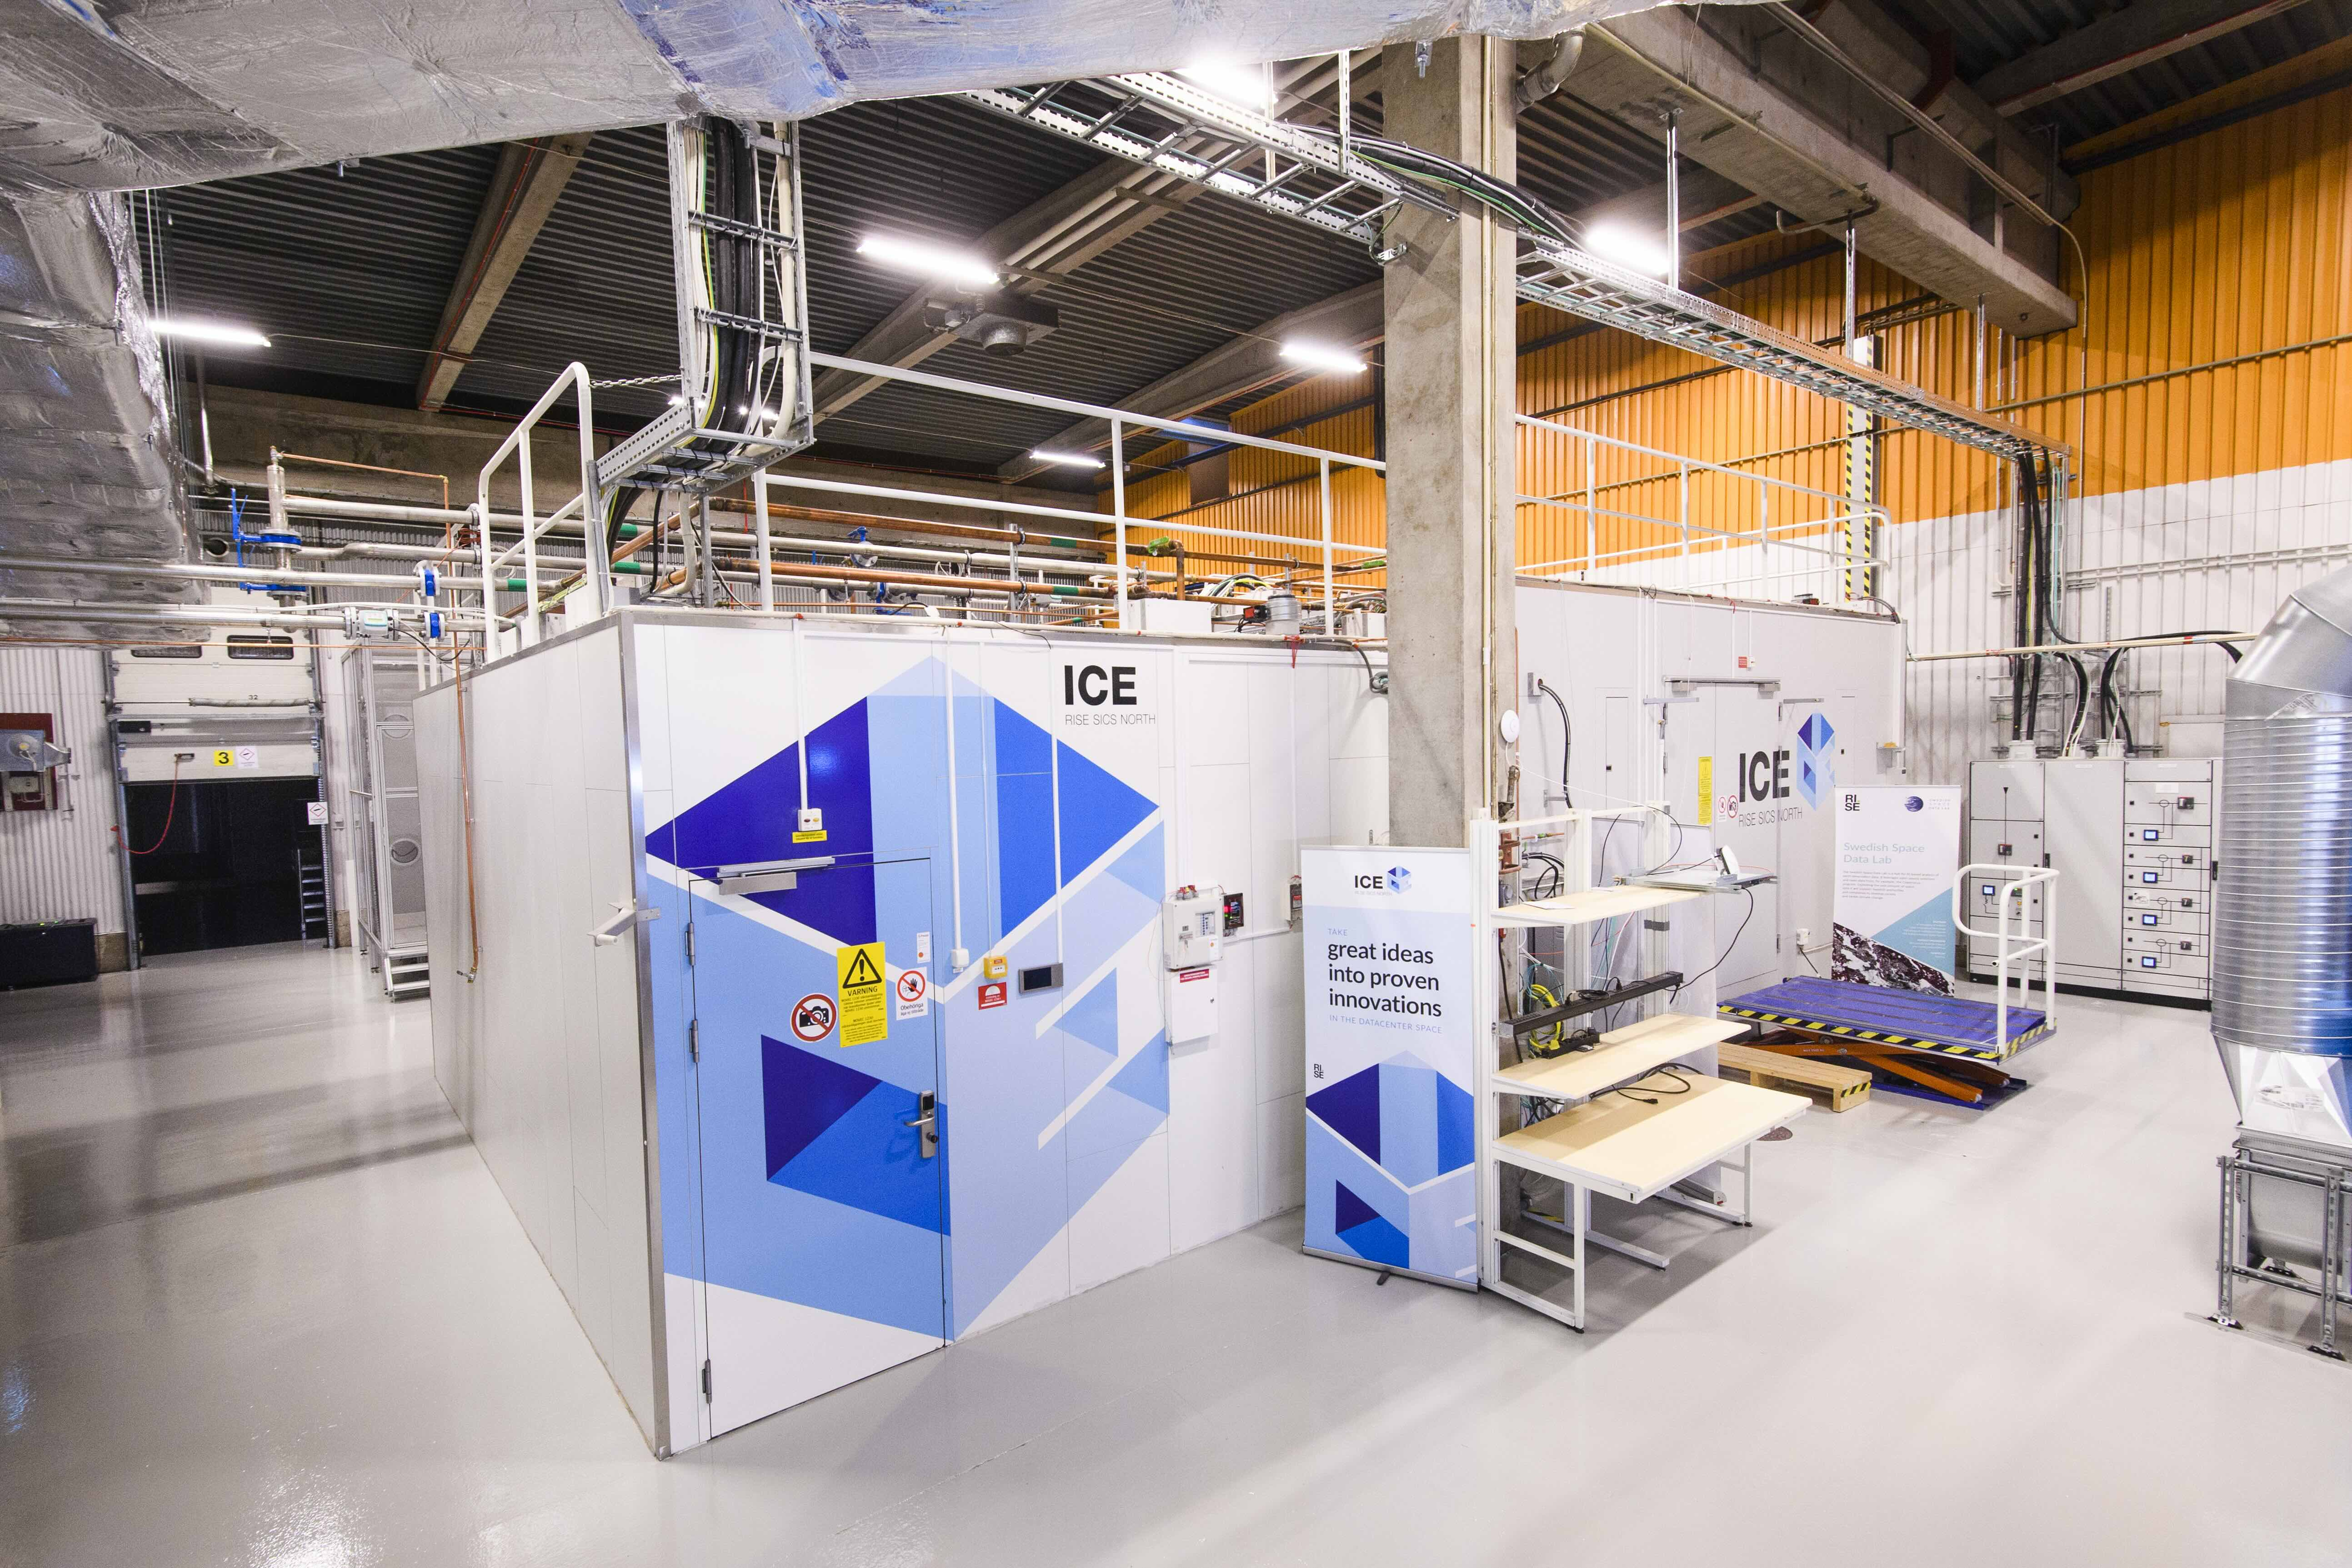
\includegraphics{images/datacenter.jpeg}}

% The optional short title keeps the content-slide footer compact.
\title[Physics-Informed PCE]{Physics-Informed Polynomial Chaos Expansion for a Thermal Digital Twin of a Data Center}
\subtitle{}
\author[Yagiz Koc / Ina Dzingarska]{Yagiz Koc \and Ina Dzingarska}
\institute{}
\date{}

\begin{document}

% Native RWTH photo cover; the local overlay credits the image on the cover itself.
\begingroup
\addtobeamertemplate{title page}{}{%
  \begin{tikzpicture}[remember picture,overlay]
    \node[anchor=south east,fill=white,fill opacity=0.9,text opacity=1,
      inner sep=0.6mm,font=\fontsize{4}{5}\selectfont,text=black!80]
      at ([xshift=-2mm,yshift=\dimexpr-2\paperheight/3+2mm\relax]current page.north east)
      {\href{https://www.ri.se/en/news/from-idea-to-an-internationally-recognised-innovation-environment-ice-datacenter-celebrates}
        {Photo: RISE / ICE Datacenter (17 June 2026)}};
  \end{tikzpicture}%
}
\maketitle[titlegraphic=2:3]
\endgroup

% Five introduction slides; subsection entries create PDF navigation only.
% Project aims and architecture are proposed, not claims of completed hardware control.
\section{Introduction}
\subsection{Motivation and Context}

\begin{frame}[more-space]{Introduction\enspace|\enspace Motivation and Context}
  \begin{columns}[T,onlytextwidth]
    \column{0.31\textwidth}
      \datametric{7\,\% to $>30$\,\%}{Cooling share of facility electricity}
      \smallskip
      {\footnotesize Efficient hyperscale to less-efficient\\enterprise facilities; IEA estimates.}
    \column{0.65\textwidth}
      \dataheading{Cooling links energy, performance and reliability}
      More CPU power $\rightarrow$ more heat\\
      More cooling $\rightarrow$ additional electricity use\\
      Excess temperature $\rightarrow$ throttling and reliability risks
  \end{columns}

  \medskip
  \begin{columns}[T,onlytextwidth]
    \column{0.315\textwidth}
      \begin{beamercolorbox}[sep=2mm,wd=\linewidth]{data panel}
        \dataheading{Computing capacity}
        \footnotesize
        More available CPU power\\
        Within the thermal budget
      \end{beamercolorbox}
    \column{0.315\textwidth}
      \begin{beamercolorbox}[sep=2mm,wd=\linewidth]{data panel}
        \dataheading{Cooling efficiency}
        \footnotesize
        Penalize cooling effort\\
        Avoid unnecessary cooling
      \end{beamercolorbox}
    \column{0.315\textwidth}
      \begin{beamercolorbox}[sep=2mm,wd=\linewidth]{data panel}
        \dataheading{Thermal safety}
        \footnotesize
        Respect CPU temperature limits\\
        Account for predictive uncertainty
      \end{beamercolorbox}
  \end{columns}

  \medskip
  \begin{beamercolorbox}[sep=2mm,wd=\textwidth]{data panel}
    \dataheading{Project goal: safer and more efficient thermal management}
    Physics-informed, uncertainty-aware predictions\\
    $\longrightarrow$ operating decisions balancing compute, cooling and safety
  \end{beamercolorbox}

  \datasource{Context: \href{https://www.iea.org/reports/energy-and-ai/energy-demand-from-ai}{IEA, Energy and AI (2025), cooling electricity share by facility type}.
    Proposed objective: thermal management balancing computation, cooling and safety.}
\end{frame}

% Set the credit outside the frame body so the RWTH footer sees it.
% This group limits the extra footer text to the photo slide.
\begingroup
\footlinetext{\href{https://www.ri.se/en/news/from-idea-to-an-internationally-recognised-innovation-environment-ice-datacenter-celebrates}{Photo: RISE / ICE Datacenter (2026)}}
\begin{frame}[more-space]{Introduction\enspace|\enspace Motivation and Context}
  \begin{columns}[T,onlytextwidth]
    \column{0.50\textwidth}
      \dataheading{RISE ICE Datacenter / Lule\aa{}, Sweden}
      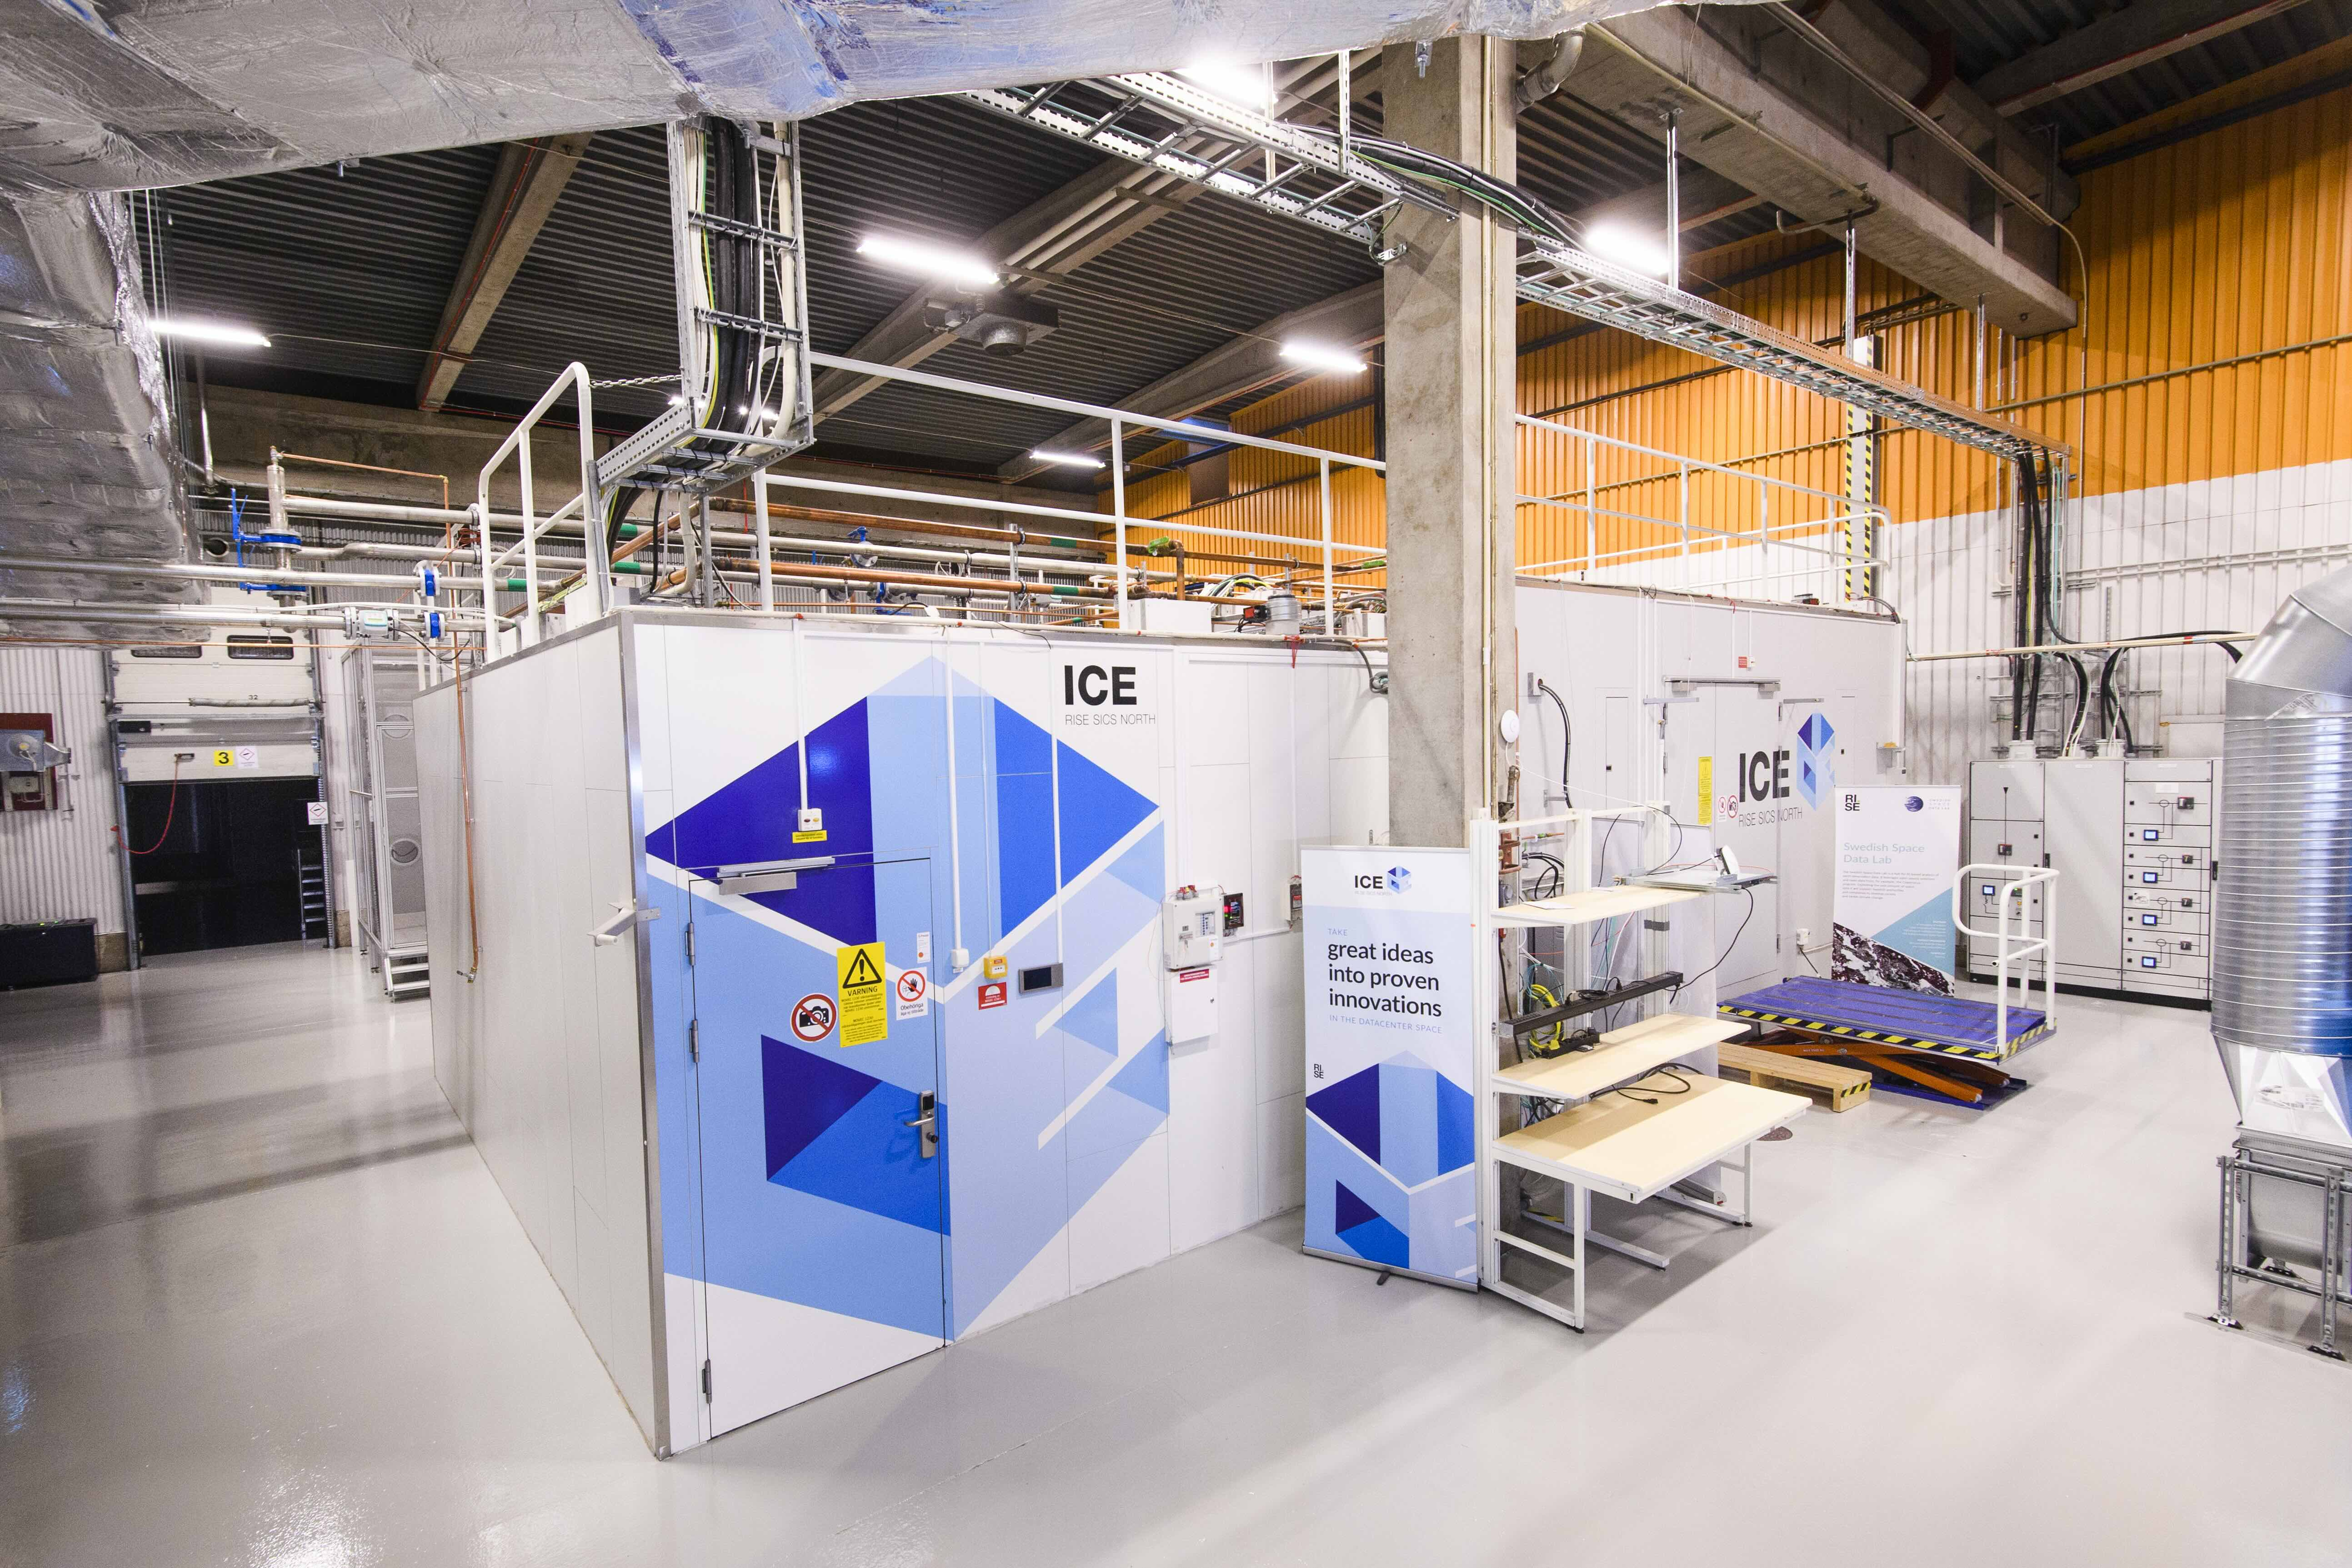
\includegraphics[width=\linewidth]{images/datacenter.jpeg}
    \column{0.46\textwidth}
      \dataheading{Experimental dataset}
      \textbf{9 OCP servers / 18 CPUs}\\
      Two Intel Xeon E5-2678 v3 CPUs per server\\
      Measurements in the RISE server wind tunnel

      \medskip
      \textbf{Original purpose}\\
      Air vs. two-phase direct-to-chip cooling\\
      Thermal performance / energy / throttling

  \end{columns}

  \datasource{Dataset: \href{https://doi.org/10.5281/zenodo.23237930}{HEATWISE / Zenodo 23237930};
    \href{https://doi.org/10.1016/j.csite.2026.107650}{Ebrahimpour Ahmadi et al., CSITE 78 (2026), 107650}.}
\end{frame}
\endgroup

\begin{frame}[more-space]{Introduction\enspace|\enspace Our Goal: An Air-cooling Actuator Digital Twin}
  \begin{columns}[T,onlytextwidth]
    \column{0.32\textwidth}
      \begin{beamercolorbox}[sep=2mm,wd=\linewidth]{data panel}
        \dataheading{Air-cooling subset}
        \textbf{1,333 records / 219 variables}\\
        \footnotesize
        Five-minute values\\
        31 Oct--5 Nov 2024

        \medskip
        \textbf{Cases 1--5}\\
        Hybrid cases excluded
      \end{beamercolorbox}

    \column{0.64\textwidth}
      \dataheading{Goal: maximize CPU power within a temperature limit}
      Optimal CPU-power and fan-power control inputs

      \medskip
      {\footnotesize
      \renewcommand{\arraystretch}{1.2}
      \begin{tabular*}{\linewidth}{@{\extracolsep{\fill}}ll@{}}
        \toprule
        \textbf{Target controls} & CPU power $P_{\mathrm{CPU}}$ / fan power $P_{\mathrm{fan}}$\\
        \textbf{Given condition} & Cooling-air inlet temperature $T_{\mathrm{in}}$\\
        \textbf{Twin prediction} & Maximum steady-state CPU temperature\\
        \bottomrule
      \end{tabular*}
      }

      \medskip
      \begin{beamercolorbox}[sep=2mm,wd=\linewidth]{data panel}
        \dataheading{Thermal constraint}
        $\widehat{T}_{\max}^{\mathrm{ss}}(P_{\mathrm{CPU}},T_{\mathrm{in}},P_{\mathrm{fan}})
          + \Delta_{\mathrm{UQ}} \leq T_{\mathrm{limit}}$
        \par\smallskip
        \footnotesize
        Predictive uncertainty margin / actuator bounds
      \end{beamercolorbox}
  \end{columns}

  \medskip
  \begin{beamercolorbox}[sep=2mm,wd=\textwidth]{data panel}
    \footnotesize
    \textbf{Computing capacity}\quad Maximize available CPU power without exceeding the thermal limit\\
    \textbf{Cooling efficiency}\quad Penalize cooling effort when selecting feasible operating points
  \end{beamercolorbox}

  \datasource{Proposed offline optimization; live actuation conceptual.
    Current data: raw fan signal with unverified unit; physical fan-power calibration required.
    Subset: dataset README and exploratory audit.}
\end{frame}

\subsection{Why a Digital Twin?}

\begin{frame}[more-space]{Introduction\enspace|\enspace Why a Digital Twin?}
  \dataheading{A measured system linked to predictions and operating decisions}
  \begin{center}
    \begin{tikzpicture}[
      node distance=5mm,
      stage/.style={fill=rwth-blue-100!6,inner sep=2mm,text width=39mm,
        minimum height=19mm,align=left,font=\footnotesize},
      >={Latex[length=2mm]}
    ]
      \node[stage] (measurements) {\textbf{Server measurements}\\
        CPU power / inlet temperature\\
        Raw fan signal\\
        Steady-state observations};
      \node[stage,right=of measurements] (surrogate) {\textbf{Proposed PI-PCE surrogate}\\
        Steady-state CPU $T_{\max}$\\
        Thermal-resistance loss\\
        Uncertainty + Sobol analysis};
      \node[stage,right=of surrogate] (decisions) {\textbf{Constrained decisions}\\
        CPU power vs. cooling effort\\
        Thermal + actuator limits\\
        Uncertainty-aware optimization};
      \draw[->,thick,rwth-blue-100] (measurements) -- (surrogate);
      \draw[->,thick,rwth-blue-100] (surrogate) -- (decisions);
    \end{tikzpicture}
  \end{center}

  \smallskip
  \begin{columns}[T,onlytextwidth]
    \column{0.315\textwidth}
      \dataheading{Fast optimization / control loop}
      \footnotesize
      Rapid surrogate evaluations\\
      Candidate operating setpoints
    \column{0.315\textwidth}
      \dataheading{Independent thermal safety}
      \footnotesize
      Measured-temperature checks\\
      Override / safe fallback actions
    \column{0.315\textwidth}
      \dataheading{Slower model-updating loop}
      \footnotesize
      New steady-state measurements\\
      Surrogate updates + revalidation
  \end{columns}

  \medskip
  \begin{beamercolorbox}[sep=2mm,wd=\textwidth]{data warning}
    \footnotesize
    \textbf{Scope}\quad Offline analysis, surrogate development, validation, UQ, sensitivity and optimization\\
    \textbf{Live hardware control}\quad Conceptual architecture; no experimental control demonstration
  \end{beamercolorbox}

  \datasource{Proposed project architecture. PCE = Polynomial Chaos Expansion;
    UQ = uncertainty quantification; Sobol analysis = variance-based input sensitivity.
    Cooling input retained as a raw signal until its unit is verified.}
\end{frame}

\subsection{Why not Synthetic Data?}

\begin{frame}[more-space]{Introduction\enspace|\enspace Why not Synthetic Data?}
  \dataheading{Project choice: anchor the model in measured server behavior}
  \begin{columns}[T,onlytextwidth]
    \column{0.48\textwidth}
      \begin{beamercolorbox}[sep=2.5mm,wd=\linewidth]{data warning}
        \dataheading{Training on simulator-generated targets}
        \textbf{Assumptions become the training reference}\\
        \footnotesize
        Thermal parameters / cooling boundary conditions\\
        Fan calibration / sensor and model discrepancy

        \medskip
        \textbf{More samples, same potential model bias}\\
        Simulator-only validation: limited hardware evidence
      \end{beamercolorbox}

    \column{0.48\textwidth}
      \begin{beamercolorbox}[sep=2.5mm,wd=\linewidth]{data panel}
        \dataheading{Experimental measurements + physics}
        \textbf{Observed response of the real servers}\\
        \footnotesize
        Load changes / cooling interactions / variability\\
        Independent measurement-based validation

        \medskip
        \textbf{Physics as guidance for the PCE}\\
        Thermal-resistance loss for plausible predictions
      \end{beamercolorbox}
  \end{columns}

  \medskip
  \begin{beamercolorbox}[sep=2mm,wd=\textwidth]{data panel}
    \dataheading{A supplementary role for synthetic data}
    \footnotesize
    Calibrated, validated simulators $\rightarrow$ augmentation and scenario tests\\
    Hardware evidence remains essential for thermal-safety validation
  \end{beamercolorbox}

  \medskip
  {\footnotesize\textbf{Next:} experimental coverage, measurement limitations and steady-state selection.}

  \datasource{Project rationale. Experimental-data constraints: dataset README, DATA\_DICTIONARY.csv and exploratory audit.
    Training and validation strategy: proposed project work.}
\end{frame}

% Standalone PCE introduction; the remaining Model chapter stays in model.tex.
\begin{frame}[more-space]{Model\enspace|\enspace Polynomial Chaos Expansion}
  \begin{beamercolorbox}[sep=2mm,wd=\textwidth]{data panel}
    \footnotesize
    A \textbf{Polynomial Chaos Expansion (PCE)} approximates a response as a
    weighted sum of orthonormal polynomial terms.
    \[
      \widehat{T}_{\max}^{\mathrm{ss}}(\mathbf{x})
      = \sum_{|\boldsymbol{\alpha}|\leq p}
        c_{\boldsymbol{\alpha}}\,\Psi_{\boldsymbol{\alpha}}(\boldsymbol{\xi})
    \]
    $c_{\boldsymbol{\alpha}}$: fitted weights; $\Psi_{\boldsymbol{\alpha}}$: polynomial terms;
    $p$: maximum total polynomial degree; $\boldsymbol{\xi}$: scaled inputs.
  \end{beamercolorbox}
  \smallskip
  \begin{columns}[T,onlytextwidth]
    \column{0.48\textwidth}
      \footnotesize
      \textbf{Inputs}\par
      Total CPU power [W]\par
      Inlet air temperature [${}^\circ$C]\par
      Raw fan signal [unit unverified]

    \column{0.49\textwidth}
      \footnotesize
      \textbf{Outputs}\par
      Maximum of the \textbf{18 CPU temperature averages} over the same
      selected steady interval [${}^\circ$C].
  \end{columns}
  \smallskip
  \begin{columns}[c,onlytextwidth]
    \column{0.78\textwidth}
      \begin{beamercolorbox}[sep=2mm,wd=\linewidth]{data panel}
        \footnotesize
        We use \textbf{UQLab} library of ETH Z\"urich for the input models and as our chosen
        PCE framework.\par
        \smallskip
        It provides polynomial bases, regression, UQ and Sobol sensitivity tools
      \end{beamercolorbox}
    \column{0.18\textwidth}
      \centering
      \href{https://www.uqlab.com/}{
\includegraphics[width=16mm,height=16mm,keepaspectratio]{images/uqlab.png}}
  \end{columns}
  \datasource{Sources: \href{https://www.uqlab.com/}{UQLab, ETH Z\"urich}}
\end{frame}

% Sources: data/raw/README.md, CASES.csv, DATA_DICTIONARY.csv;
% results/audit/report.md, quality_summary.json and tables/.
% Four context slides followed by the preprocessing-results subsection.
\section{Input Data}

\begin{frame}[more-space]{Input Data\enspace|\enspace Operating cases and model variables}
  \begin{columns}[T,onlytextwidth]
    \column{0.47\textwidth}
      \dataheading{Measured variables}
      {\footnotesize
      \renewcommand{\arraystretch}{1.25}
      \setlength{\tabcolsep}{4pt}
      \begin{tabular*}{\linewidth}{@{\extracolsep{\fill}}lr@{}}
        \toprule
        \textbf{Model input} & \textbf{Observed range}\\
        \midrule
        Total CPU power & 329--2,312 W\\
        Inlet air temperature & 23.4--46.4\,${}^\circ$C\\
        Raw fan signal & 0.117--0.766\\
        \midrule
        \textbf{Response} & \\
        Maximum CPU temperature & 36--95\,${}^\circ$C\\
        \bottomrule
      \end{tabular*}
      \smallskip
      Marginal ranges include transition rows.\\
      Fan signal: original scale, unit unverified.
      }

    \column{0.50\textwidth}
      \dataheading{Five operating regimes}
      {\footnotesize
      \renewcommand{\arraystretch}{1.12}
      \setlength{\tabcolsep}{4pt}
      \begin{tabular*}{\linewidth}{@{\extracolsep{\fill}}lrrr@{}}
        \toprule
        \textbf{Case} & \textbf{Inlet} & \textbf{DP} & \textbf{Rows}\\
        & $[{}^\circ\mathrm{C}]$ & $[\mathrm{kPa}]$ & \\
        \midrule
        \casekey{caseone}{1}   & 25 &  2 & 249\\
        \casekey{casetwo}{2}   & 35 &  4 & 304\\
        \casekey{casethree}{3} & 45 &  6 & 237\\
        \casekey{casefour}{4}  & 45 &  8 & 309\\
        \casekey{casefive}{5}  & 45 & 10 & 209\\
        \bottomrule
      \end{tabular*}
      \smallskip
      Inlet and DP: \textbf{setpoints}; DP $\ne$ fan power.\\
      \texttt{stress-ng}: \textbf{100 / 75 / 50 / 25\,\% / idle}\\
      Case labels: curated constant-setpoint stretches
      }
  \end{columns}

  \medskip
  \begin{beamercolorbox}[sep=1.3mm,wd=\textwidth]{data panel}
    \footnotesize
    \textbf{Modeling subset}\quad Select steady-state intervals; curated case labels alone are insufficient.\\
    \textbf{Strict maximum}\quad All CPU temperature readings required; no missing-sensor imputation.
  \end{beamercolorbox}

  \datasource{Sources: CASES.csv; results/audit/report.md, case\_summary.csv and numerical\_ranges.csv.
    Marginal ranges describe observations, not a fully tested operating box.}
\end{frame}

\subsection{Problems with the dataset}

\begin{frame}[more-space]{Input Data\enspace|\enspace Problems with the dataset}
  \begin{columns}[T,onlytextwidth]
    \column{0.46\textwidth}
      \dataheading{Observed inlet / fan combinations}
      \centering
      % Panel (a) of the existing vector figure; other panels and the shared
      % legend are clipped only at display time. Source PDF stays unchanged.
      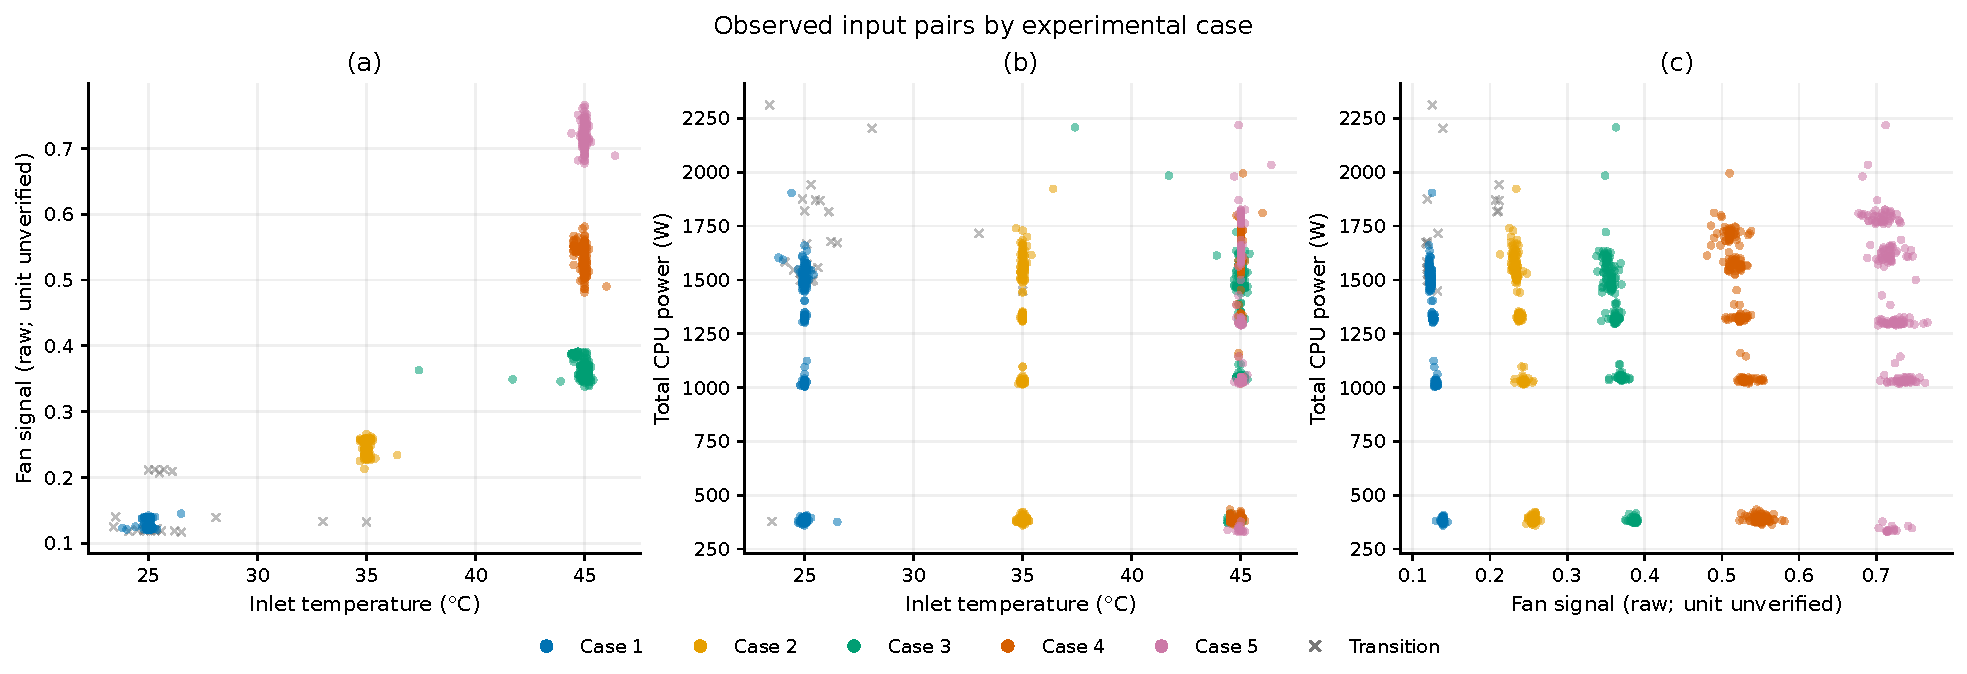
\includegraphics[width=\linewidth,height=49mm,keepaspectratio,
        trim=0bp 24bp 634bp 40bp,clip]
        {../../results/audit/figures/pairwise_input_scatter.pdf}
      \par\smallskip
      {\footnotesize
        \casekey{caseone}{1}\quad\casekey{casetwo}{2}\quad
        \casekey{casethree}{3}\quad\casekey{casefour}{4}\quad
        \casekey{casefive}{5}\quad{\color{black!50}$\times$}\,transition
      }

    \column{0.51\textwidth}
      \begin{beamercolorbox}[sep=2mm,wd=\linewidth]{data panel}
        \dataheading{1. Sparsity}
        {\large\color{rwth-blue-100}\bfseries 31 / 125}\;occupied grid cells\par
        \smallskip
        Five bins per input; binning-dependent diagnostic\\
        Five trajectories; no full factorial design\\
        \textbf{Untested:} high fan signal at $25\,{}^\circ$C
      \end{beamercolorbox}

      \medskip
      \begin{beamercolorbox}[sep=2mm,wd=\linewidth]{data warning}
        \dataheading{2. Unverified unit of fan signal}
        Dictionary confidence: \textbf{low}\\
        Retain raw scale; no W / kW conversion\\
        Calibrated fan-energy costs unavailable\\
        \textbf{Needed:} confirmation from data owners
      \end{beamercolorbox}

      \medskip
      {\footnotesize\textbf{Modeling:} validate new combinations before optimization.}
  \end{columns}

  \datasource{Sources: exploratory audit, coverage\_grid.csv and DATA\_DICTIONARY.csv.
    Figure: pairwise\_input\_scatter.pdf (a). Grid occupancy: labeled cases only;
    resolution-dependent diagnostic, not a validated operating boundary.}
\end{frame}

\begin{frame}[more-space]{Input Data\enspace|\enspace Problems with the dataset}
  \begin{columns}[T,onlytextwidth]
    \column{0.66\textwidth}
      \dataheading{Observed correlations between the model inputs}
      % Use the existing vector figure in place; trim its redundant top title.
      % Both correlation matrices, tick labels, and the color scale are retained.
      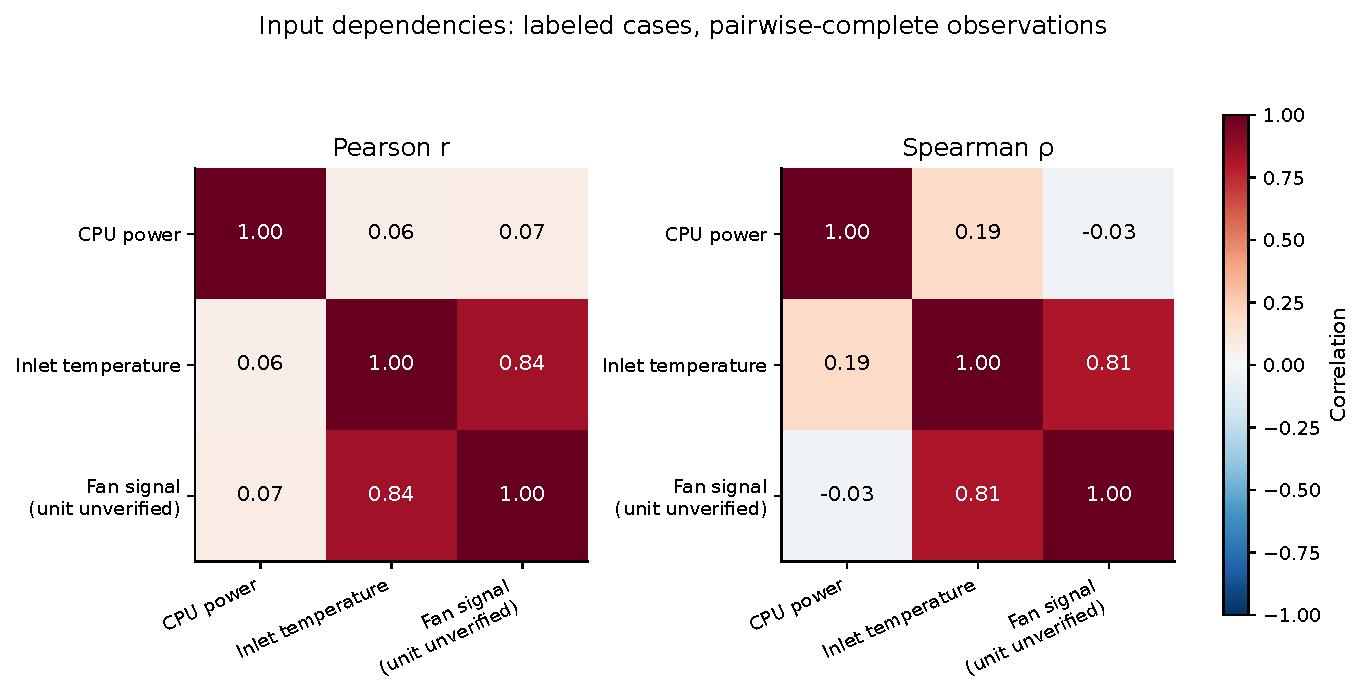
\includegraphics[width=\linewidth,trim=0bp 0bp 0bp 35bp,clip]
        {../../results/audit/figures/input_correlation_matrix.pdf}
      \par\smallskip
      {\footnotesize
        Pearson: linear / Spearman: rank correlation\\
        Labeled cases 1--5; pairwise-complete observations ($n=1{,}308$)
      }

    \column{0.31\textwidth}
      \begin{beamercolorbox}[sep=2mm,wd=\linewidth]{data panel}
        \dataheading{3. Input Dependence}
        \textbf{Fan signal / inlet temperature}\par
        \smallskip
        {\large\color{rwth-blue-100}\bfseries $r=0.84$\quad $\rho=0.81$}\par
        \smallskip
        Shared experimental case design\\
        Strong pooled association
      \end{beamercolorbox}

      \medskip
      \dataheading{Implications for PCE / UQ}
      \footnotesize
      Independent marginal sampling\\
      $\rightarrow$ untested input combinations

      \medskip
      Review independence assumptions\\
      before classical PCE / Sobol analysis

      \medskip
      \textbf{Near-zero correlation}\\
      $\ne$ statistical independence
  \end{columns}

  \datasource{Sources: results/audit/report.md and tables/input\_dependencies.csv.
    Figure: input\_correlation\_matrix.pdf, referenced directly from results/audit/figures/.
    Pooled relationships include between-case changes; correlation does not establish causality.}
\end{frame}

\subsection{Need for preprocessing and steady-stateness of the data}

\begin{frame}[more-space]{Input Data\enspace|\enspace Need for preprocessing and steady-stateness of the data}
  \begin{columns}[T,onlytextwidth]
    \column{0.56\textwidth}
      \dataheading{Load steps and thermal response}
      % Display panels (a) and (d) from the same existing time-series PDF.
      % The shared case colors and time axis are retained; no data are altered.
      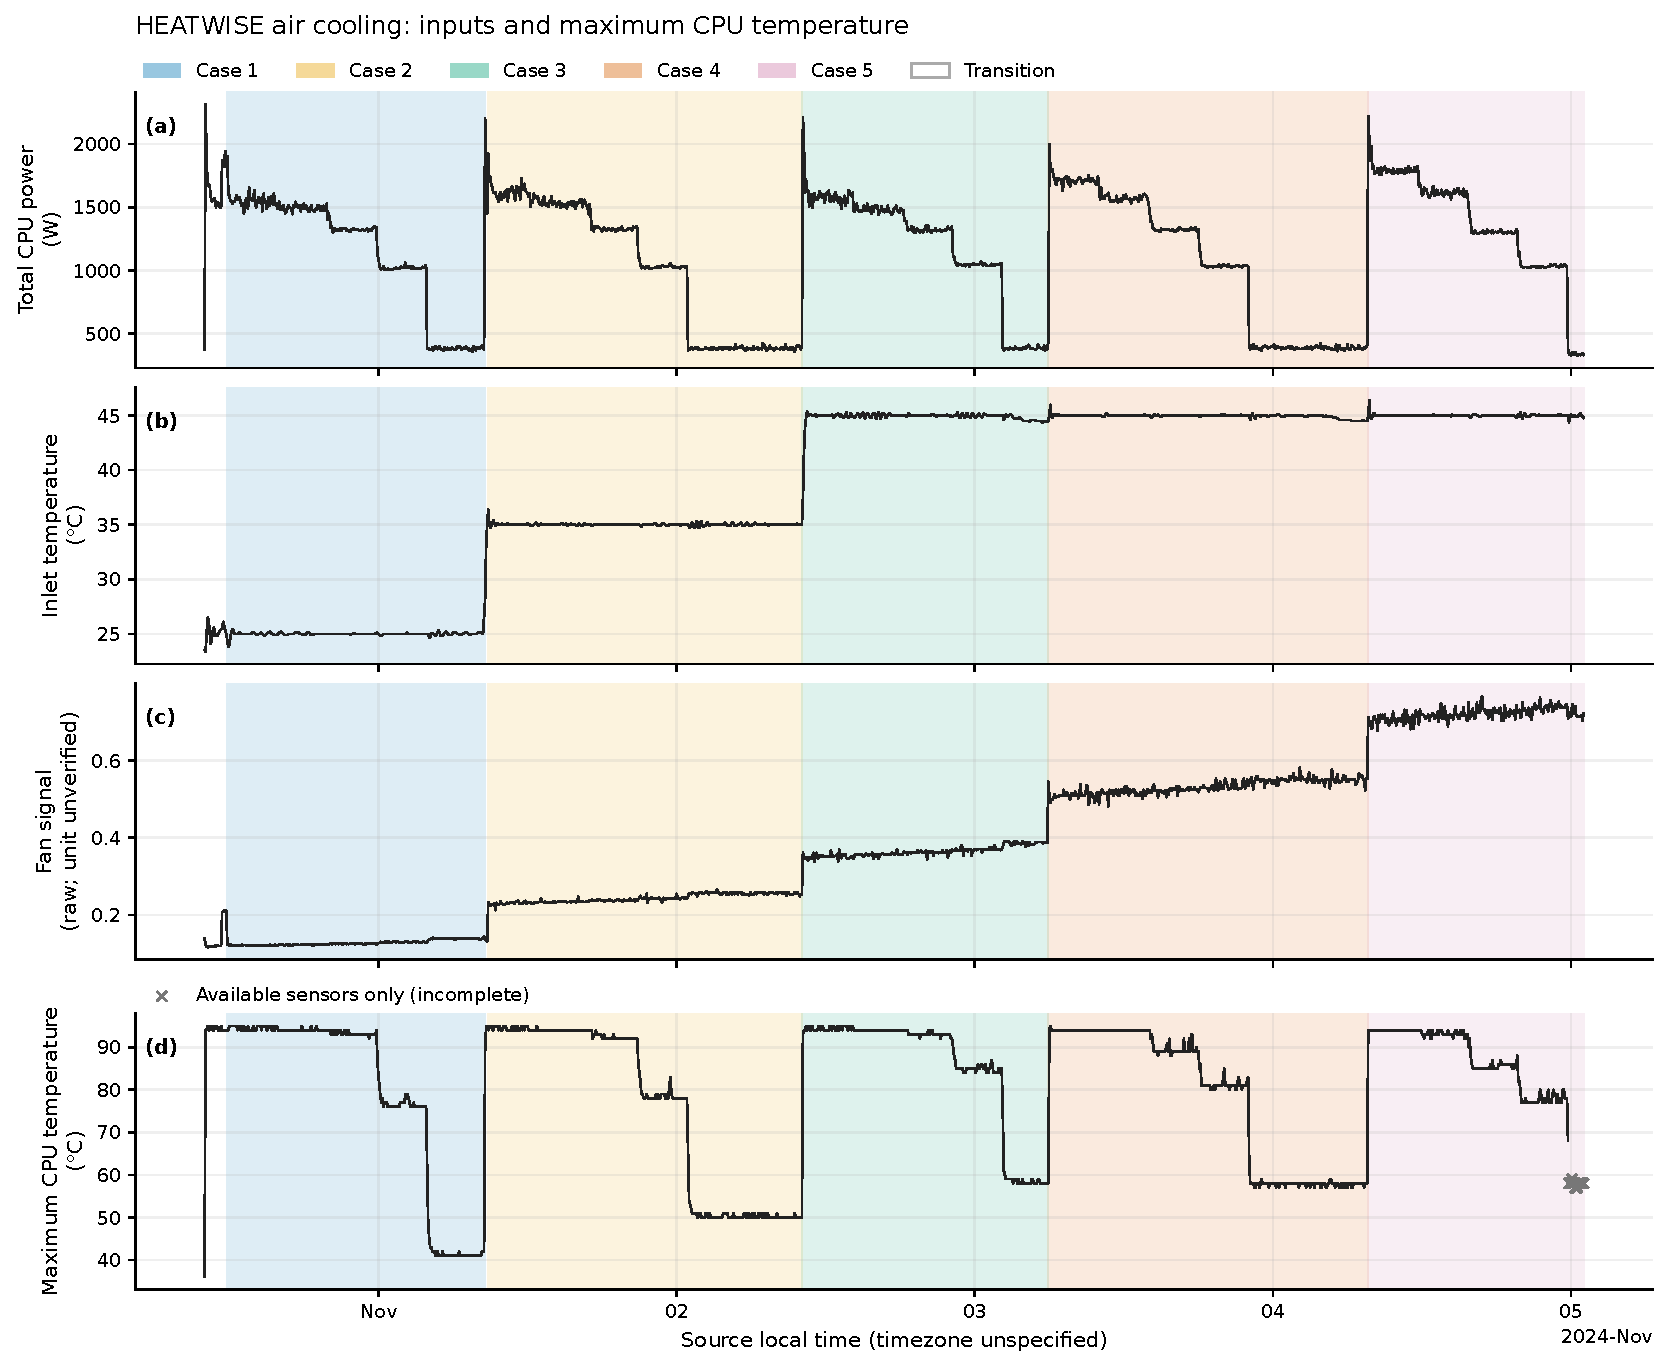
\includegraphics[width=\linewidth,trim=0bp 478bp 0bp 22bp,clip]
        {../../results/audit/figures/inputs_and_max_temperature_timeseries.pdf}
      \par\vspace{1mm}
      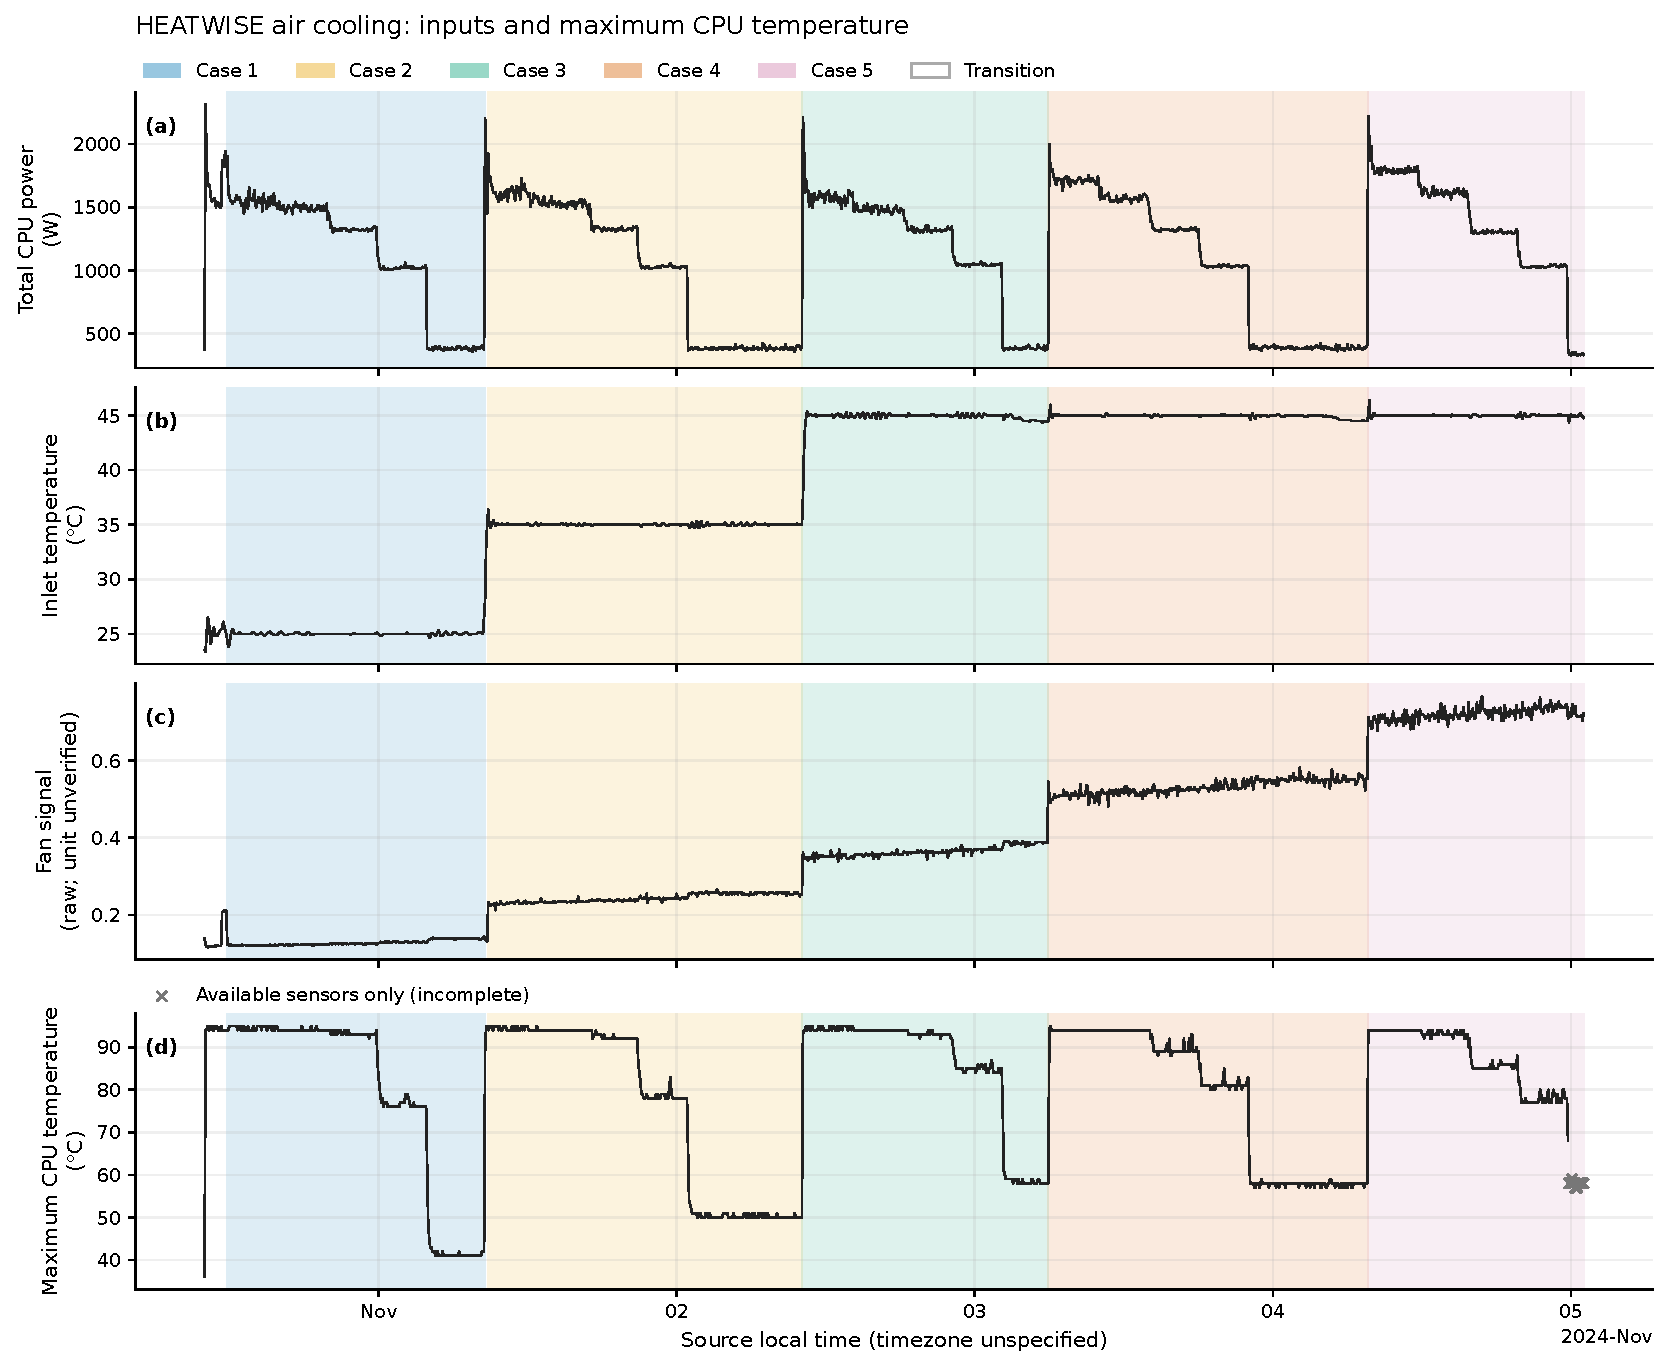
\includegraphics[width=\linewidth,trim=0bp 0bp 0bp 472bp,clip]
        {../../results/audit/figures/inputs_and_max_temperature_timeseries.pdf}
      \par\medskip
      {\footnotesize
        \textbf{25} unlabeled start-up / transition rows\\
        \textbf{15} rows with incomplete CPU readings\\
        Strict $T_{\max}$: all 18 sensors required
      }

    \column{0.41\textwidth}
      \begin{beamercolorbox}[sep=2mm,wd=\linewidth]{data panel}
        \dataheading{Preprocessing before fitting}
        \footnotesize
        Separate start-up / transition rows\\
        Flag incomplete CPU temperature readings\\
        Derive strict maxima from complete sensor sets\\
        Preserve raw data; no sensor imputation
      \end{beamercolorbox}

      \medskip
      \begin{beamercolorbox}[sep=2mm,wd=\linewidth]{data panel}
        \dataheading{Select steady-state intervals}
        \footnotesize
        Case label $\ne$ thermal equilibrium\\
        Exclude settling after load / setpoint changes\\
        Stable inputs \textbf{and} CPU temperatures\\
        Paper: $\geq 10$ min steady-state averages\\
        Five-minute sampling / averaging: unclear
      \end{beamercolorbox}
  \end{columns}

  \datasource{Sources: data/raw/README.md; results/audit/report.md and quality\_summary.json.
    Figure: inputs\_and\_max\_temperature\_timeseries.pdf, panels (a) and (d). Implemented selection and results follow.}
\end{frame}

% Existing selection figure is included directly, without changing data.
\subsection{Preprocessing results}
\definecolor{selectiongreen}{HTML}{009E73}

\begin{frame}[more-space]{Input Data\enspace|\enspace Preprocessing results}
  \begin{columns}[T,onlytextwidth]
    \column{0.56\textwidth}
      \dataheading{Selected approximately steady intervals}
      \centering
      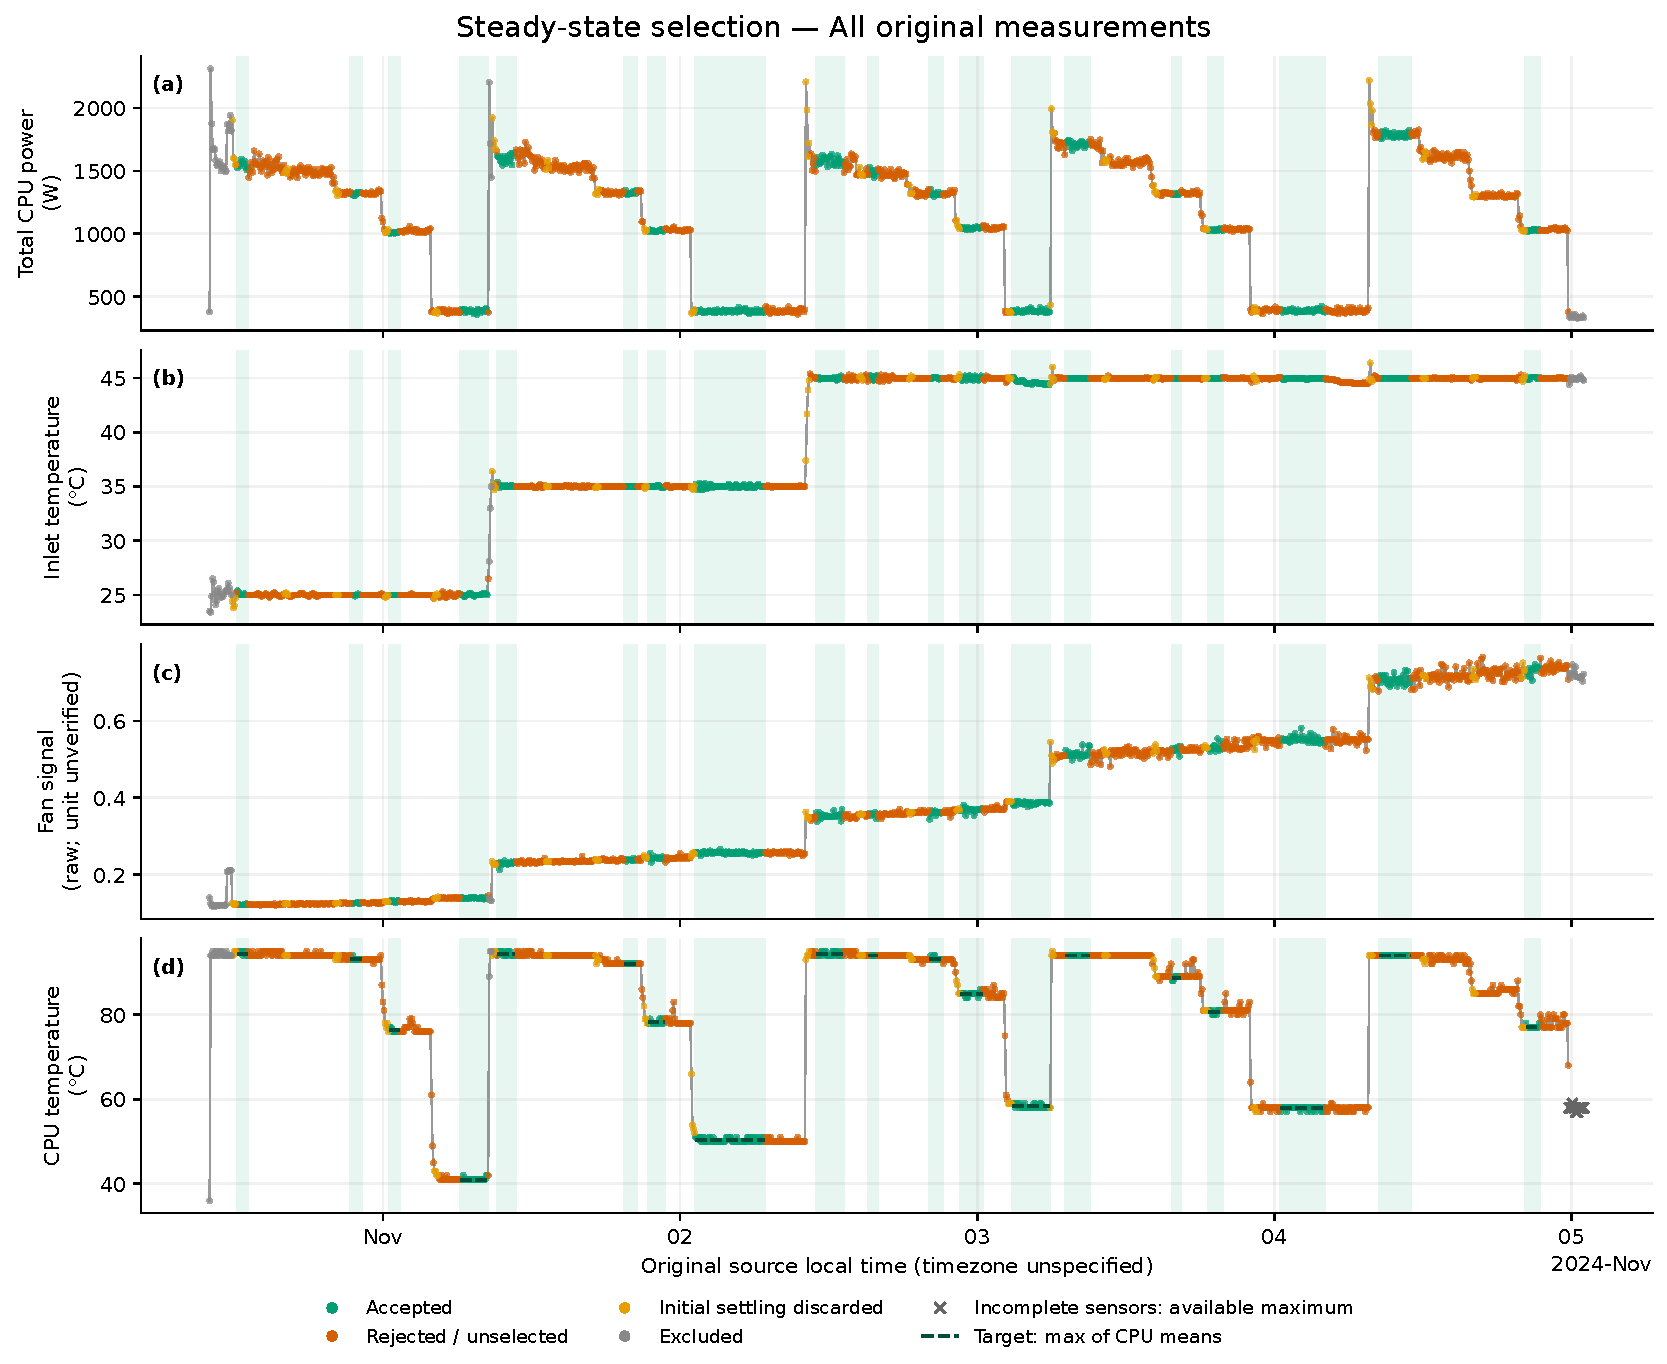
\includegraphics[width=\linewidth,height=50mm,keepaspectratio]
        {../../results/preprocessing/figures/selection_overview.pdf}
      \par\smallskip
      {\small\color{selectiongreen}\textbf{One green band = one processed observation.}}
      \par\smallskip
      {\footnotesize \textbf{60-minute dwell: 14 observations} (backup).}

    \column{0.41\textwidth}
      \begin{beamercolorbox}[sep=2mm,wd=\linewidth]{data panel}
        {\color{rwth-blue-100}\fontsize{22}{25}\selectfont\bfseries 19}\par
        \textbf{operating observations}\par
      \end{beamercolorbox}
      \medskip
      \dataheading{Each observation contains:}
      \footnotesize
      \[
        \Bigl(
          \underbrace{\bar P_{\mathrm{CPU}},\,\bar T_{\mathrm{inlet}},\,\bar F}_{\text{three inputs}},\;
          \underbrace{\max_{j=1,\ldots,18}\bar T_j}_{\text{temperature target}}
        \Bigr)
      \]
      Interval averages; $j=1,\ldots,18$ indexes CPUs.
      \par\smallskip
      \begin{beamercolorbox}[sep=1.5mm,wd=\linewidth]{data warning}
        \dataheading{Our starting choice: degrees 1 and 2}
        \footnotesize
        \begin{itemize}
          \item Full bases: \textbf{4 / 10 coefficients}; cubic: 20 ($>19$).
          \item Quadratic design: $\kappa_2\approx702$; coefficients may be unstable.
          \item Higher degrees need sparsity / regularization; validate either choice.
        \end{itemize}
      \end{beamercolorbox}
  \end{columns}
\end{frame}

% Assumed reference distributions; experimental data are unchanged.
\subsection{Input distributions}

\begin{frame}[more-space]{Input Data\enspace|\enspace Input distributions}
  \dataheading{Uniform inputs: equal weight across each observed range}
  \small
  Bounds come from the \textbf{19 processed observations}.
  \par\medskip
  {\renewcommand{\arraystretch}{1.35}
  \begin{tabular*}{\textwidth}{@{\extracolsep{\fill}}lrrl@{}}
    \toprule
    \textbf{Input} & \textbf{Lower bound} & \textbf{Upper bound} & \textbf{Unit}\\
    \midrule
    Total CPU power & 384.735 & 1,786.226 & W\\
    Inlet air temperature & 25.000 & 45.056 & ${}^\circ$C\\
    Raw fan signal & 0.121636 & 0.730571 & unverified\\
    \bottomrule
  \end{tabular*}}
  \smallskip
  \begin{beamercolorbox}[sep=1.5mm,wd=\textwidth]{data panel}
    \dataheading{Scale each parameter to $[-1,1]$}
    \footnotesize
    \setlength{\abovedisplayskip}{2pt}
    \setlength{\belowdisplayskip}{2pt}
    \[
      x_i\in[a_i,b_i]\quad\Longrightarrow\quad
      \xi_i=2\frac{x_i-a_i}{b_i-a_i}-1
    \]
    Lower bound $\mapsto-1$; midpoint $\mapsto0$; upper bound $\mapsto1$.\par
    Uniform reference inputs become $\mathcal U(-1,1)$: Use a normalized \textbf{Legendre} basis as the orthonormal polynomial family for the PCE.
  \end{beamercolorbox}
\end{frame}

\subsection{Digital Twin Definition}

\begin{frame}[more-space]{Summary: Digital Twin Definition}
  {\normalfont\small
  \renewcommand{\arraystretch}{1.35}
  \setlength{\tabcolsep}{4pt}
  \begin{tabular}{@{}p{0.23\textwidth}p{0.73\textwidth}@{}}
    \toprule
    \textbf{Element} & \textbf{Our thermal digital twin}\\
    \midrule
    \textbf{Model} & \mdseries
      Planned: PCE vs PI-PCE with monotonicity constraints; degrees 1 / 2\\
    \midrule
    \textbf{Parameters} & \mdseries
      Surrogate coordinates: CPU power $P$, fan signal $F$, inlet temperature $T$\\
    \midrule
    \textbf{Inputs} & \mdseries
      Surrogate: $(P,T,F)$; controller disturbance: inlet temperature\\
    \midrule
    \textbf{Outputs} & \mdseries
      Surrogate: maximum interval-mean CPU temperature; controller: proposed $(P,F)$\\
    \midrule
    \textbf{Measurement operator} & \mdseries
      18 CPU sensors, every 5 min; $\mathcal H=\max_{j=1,\ldots,18}\overline{T}_j$ over an approximately steady period\\
    \midrule
    \textbf{Observables} & \mdseries
      19 approximately steady temperature targets\\
    \midrule
    \textbf{Quantity of interest} & \mdseries
      CPU / fan choice within a validated domain and error bound; hardware protects peaks\\
    \bottomrule
  \end{tabular}
  }
\end{frame}


\section{Model}
\subsection{Adding Physics: Physics-Informed PCE}

\begin{frame}[more-space]{Model\enspace|\enspace Adding Physics: Physics-Informed PCE}
  \dataheading{A simple thermal-resistance model as physical guidance}
  \begin{beamercolorbox}[sep=2mm,wd=\textwidth]{data panel}
    \footnotesize
    At equilibrium, temperature rise is approximated by heat generation
    multiplied by an effective thermal resistance:
    \[
      T_{\mathrm{phys}}=T_{\mathrm{inlet}}+\Delta T_0
        +P_{\mathrm{CPU}}R_{\mathrm{th}}(F),
      \qquad F=P_{\mathrm{fan,raw}}>0,
    \]
    \[
      R_{\mathrm{th}}(F)=R_0+K\left(\frac{F}{F_{\mathrm{ref}}}\right)^{-\gamma}.
    \]
  \end{beamercolorbox}
  \medskip
  \begin{columns}[T,onlytextwidth]
    \column{0.48\textwidth}
      \dataheading{Meaning of the parameters}
      \footnotesize
      $R_0\geq0$: resistance remaining at strong cooling.\par
      $K\geq0$: additional resistance at reference cooling.\par
      $\gamma>0$: how resistance decreases with cooling.\par
      $\Delta T_0$: fitted temperature offset.\par
      \smallskip
      $R_0,K$ have units of ${}^\circ$C/W.
    \column{0.49\textwidth}
      \dataheading{Calibration}
      \footnotesize
      Fix $F_{\mathrm{ref}}>0$ on the same raw scale so $F/F_{\mathrm{ref}}$
      is dimensionless. It is not a conversion to watts.\par
      \smallskip
      Calibrate the remaining parameters using training cases only.
      With 19 observations, check identifiability and simplify if needed.
  \end{columns}
\end{frame}

\begin{frame}[more-space]{Model\enspace|\enspace Adding Physics: Physics-Informed PCE}
  \begin{beamercolorbox}[sep=2mm,wd=\textwidth]{data panel}
    \footnotesize
    The prediction keeps the same orthonormal Legendre expansion.
    Only the objective used to learn its coefficients changes:
    \[
      \mathcal L(\mathbf c)=
      \underbrace{\frac{1}{N}\sum_{i=1}^{N}
        \left[\widehat T_{\max}(\mathbf x_i)-y_i\right]^2}_{\mathcal L_{\mathrm{data}}}
      +\lambda_{\mathrm{phys}}
      \underbrace{\frac{1}{M}\sum_{j=1}^{M}
        \left[\widehat T_{\max}(\mathbf z_j)-T_{\mathrm{phys}}(\mathbf z_j)\right]^2}
        _{\mathcal L_{\mathrm{physics}}}.
    \]
  \end{beamercolorbox}
  \medskip
  \begin{columns}[T,onlytextwidth]
    \column{0.48\textwidth}
      \dataheading{Fit measurements and encourage physics}
      \footnotesize
      $N$: training observations; $y_i$: measured targets.\par
      $M$: physics-check operating points $\mathbf z_j$.\par
      \smallskip
      Restrict checks to supported, validated operating conditions; generated
      points are not additional experimental evidence.
    \column{0.49\textwidth}
      \dataheading{Choose the physics influence}
      \footnotesize
      $\lambda_{\mathrm{phys}}\geq0$ controls the compromise.
      Zero gives the data-only baseline. Select it within training-case validation.\par
      \smallskip
      This is a loss-based idea similar to a PINN, using polynomials instead of a neural network.
  \end{columns}
\end{frame}

\begin{frame}[more-space]{Model\enspace|\enspace Adding Physics: Physics-Informed PCE}
  \begin{columns}[T,onlytextwidth]
    \column{0.48\textwidth}
      \begin{beamercolorbox}[sep=2mm,wd=\linewidth]{data panel}
        \dataheading{What it could improve}
        \footnotesize
        \begin{itemize}
          \item Encourage realistic heating and cooling trends.
          \item Potentially improve predictions with sparse data.
          \item Keep fast PCE, UQ and Sobol calculations.
        \end{itemize}
      \end{beamercolorbox}
    \column{0.49\textwidth}
      \begin{beamercolorbox}[sep=2mm,wd=\linewidth]{data warning}
        \dataheading{What it cannot guarantee}
        \footnotesize
        \begin{itemize}
          \item A penalty does not enforce exact physics.
          \item Missing input combinations remain untested.
        \end{itemize}
      \end{beamercolorbox}
  \end{columns}
  \medskip
  \begin{beamercolorbox}[sep=2mm,wd=\textwidth]{data panel}
    \dataheading{How we would decide whether it helps}
    \footnotesize
    \begin{itemize}
      \item Compare PCE and PI-PCE on the same held-out cases.
      \item Fit physics parameters and tune the loss weight using training cases only.
      \item Keep the simpler model unless accuracy and physical behavior improve.
      \item Extra tuning requires more validation.
    \end{itemize}
  \end{beamercolorbox}
\end{frame}


% Proposed UQ, sensitivity, optimization and deployment stages.
\section{Uncertainty Quantification and Sensitivity Analysis}

\begin{frame}[more-space]{UQ\enspace|\enspace Rearranging the PCE to find uncertainties w.r.t inlet air temperature}
  \footnotesize
  \setlength{\abovedisplayskip}{2pt}
  \setlength{\belowdisplayskip}{2pt}
  \setlength{\abovedisplayshortskip}{1pt}
  \setlength{\belowdisplayshortskip}{1pt}
  \begin{columns}[T,onlytextwidth]
    \column{0.51\textwidth}
      \begin{beamercolorbox}[sep=1.5mm,wd=\linewidth]{data panel}
        \dataheading{1. Insert one CPU / fan setting}
        $P=1000\,\mathrm W$, $F=0.4$. Suppose the model becomes:
        \[
          \widehat T=80+2(T_{\mathrm{inlet}}-35)
            +0.3(T_{\mathrm{inlet}}-35)^2.
        \]
      \end{beamercolorbox}
    \column{0.46\textwidth}
      \begin{beamercolorbox}[sep=1.5mm,wd=\linewidth]{data panel}
        \dataheading{2. Choose an inlet variation $\delta$}
        $\delta>0$: assumed half-width [${}^\circ$C]; range $[35-\delta,35+\delta]$.
        \[
          T_{\mathrm{inlet}}=35+\delta\xi,\qquad \xi\sim\mathcal U(-1,1)
        \]
        \[
          \Longrightarrow\quad\widehat T=80+2\delta\xi+0.3\delta^2\xi^2.
        \]
      \end{beamercolorbox}
  \end{columns}
  \smallskip
  \begin{beamercolorbox}[sep=1.5mm,wd=\textwidth]{data panel}
    \dataheading{3. Rewrite the same curve using normalized Legendre terms}
    \[
      \phi_1=\sqrt3\,\xi,\qquad
      \phi_2=\frac{\sqrt5}{2}(3\xi^2-1)
      \quad\Longrightarrow\quad
      \xi=\frac{\phi_1}{\sqrt3},\qquad
      \xi^2=\frac13+\frac{2\phi_2}{3\sqrt5}.
    \]
    \[
      \widehat T
        =\underbrace{80+0.1\delta^2}_{b_0}
             +\underbrace{2\delta/\sqrt3}_{b_1}\phi_1
             +\underbrace{0.2\delta^2/\sqrt5}_{b_2}\phi_2.
    \]
  \end{beamercolorbox}
  \smallskip
  \begin{beamercolorbox}[sep=1.5mm,wd=\textwidth]{data warning}
    \dataheading{4. Read the mean and spread for this setting}
    \[
      \mu_T=b_0=80+0.1\delta^2,\qquad
      \sigma_T=\sqrt{b_1^2+b_2^2}
        =\sqrt{4\delta^2/3+0.008\delta^4}.
    \]
  \end{beamercolorbox}
\end{frame}

\begin{frame}[more-space]{Sensitivity Analysis}
  \begin{tikzpicture}[remember picture,overlay]
    \node[anchor=center,inner sep=0pt] at (current page.center) {%
      \begin{minipage}{\textwidth}
  {\normalfont\small
  \renewcommand{\arraystretch}{1.3}
  \begin{tabular}{@{}p{0.19\textwidth}p{0.77\textwidth}@{}}
    \toprule
    \textbf{Coefficient} & \textbf{At a fixed CPU / fan setting}\\
    \midrule
    $b_0(P,F)$ & Average predicted CPU temperature\\
    $b_1(P,F)$ & Strength and direction of the linear response to air inlet temperature changes\\
    $b_2(P,F)$ & Strength and direction of the curvature in the air inlet temperature response\\
    \bottomrule
  \end{tabular}}
  \medskip
  \begin{itemize}
    \small
    \item Compare settings using the \textbf{same inlet range / distribution}. $b_1^2,b_2^2$ split inlet variance into linear / curvature parts.
    \item Only inlet varies here: its Sobol index is 1 if variance is nonzero. \textbf{This cannot rank the three inputs.}
    \item Full total-degree 2: $b_1$ can vary with $P,F$; $b_2$ is constant. Degree 1: $b_1$ is constant and $b_2=0$.
  \end{itemize}
      \end{minipage}%
    };
  \end{tikzpicture}
\end{frame}

\section{Optimization Problem: Soft-constrained optimal control}

\begin{frame}[more-space]{Optimization Problem: Soft-constrained optimal control}
  \dataheading{Trade computing capacity against cooling effort}
  {\footnotesize
  At measured inlet temperature, choose CPU power $P$, fan signal $F$ and
  thermal slack $s_T\geq0$. Proposed formulation:
  \[
    \begin{aligned}
      \max_{P,F,s_T}\quad & P-\lambda_F F-\rho s_T^2\\
      \text{subject to}\quad
      &\mu_T(P,F)+k\sigma_T(P,F)
          \leq T_{\mathrm{limit}}-\Delta T_{\mathrm{safety}}+s_T,\\
      &P_{\min}\leq P\leq P_{\max},\qquad F_{\min}\leq F\leq F_{\max},\\
      &|P-P_{\mathrm{before}}|\leq\Delta P_{\max},\qquad
        |F-F_{\mathrm{before}}|\leq\Delta F_{\max},\\
      &(P,T_{\mathrm{inlet}}^{\mathrm{meas}},F)\in\mathcal D_{\mathrm{supported}},
        \qquad s_T\geq0.
    \end{aligned}
  \]
  }
  \begin{columns}[T,onlytextwidth]
    \column{0.48\textwidth}
      \dataheading{Meaning of the objective}
      \footnotesize
      Reward CPU power as a computing-capacity proxy; penalize cooling effort
      and thermal-target violations.\par
      \smallskip
      $\lambda_F\geq0$ sets the cooling compromise; $\rho>0$ penalizes slack.
      Weight units/scales must match the objective.
    \column{0.49\textwidth}
      \dataheading{Why this is soft-constrained}
      \footnotesize
      Positive $s_T$ allows a penalized violation of the modeled thermal target.
      Actuator limits, step limits and domain restrictions remain hard.\par
      \smallskip
      Previous CPU/fan settings appear in step constraints, not as an initial thermal state of the PCE.
  \end{columns}
  \datasource{Proposed adaptation of the notes to the agreed soft-constraint objective.
    $F=P_{\mathrm{fan,raw}}$, unit unverified; $\lambda_F F$ is not a calibrated electrical-energy cost.
    Limits, weights, disturbance law and domain rule require specification; optimization is not implemented.}
\end{frame}

\begin{frame}[more-space]{Optimization Problem: Soft-constrained optimal control}
  \dataheading{Keep the optimizer inside conditions we can defend}
  \begin{columns}[T,onlytextwidth]
    \column{0.48\textwidth}
      \dataheading{A small, fast numerical problem}
      \footnotesize
      Evaluate the surrogate repeatedly for candidate CPU/fan settings.
      Use a small constrained solver; an explicit solution is optional only
      if the final formulation permits one.\par
      \smallskip
      The nonlinear surrogate and risk term may create local optima.
      Check candidate solutions, feasibility and sensitivity to starting points.
    \column{0.49\textwidth}
      \dataheading{Data and actuation limits}
      \footnotesize
      Observed ranges are an outer boundary, not proof that every combination
      inside the box was tested. Restrict $\mathcal D_{\mathrm{supported}}$
      using coverage and validation evidence.\par
      \smallskip
      Electrical fan power may not be directly commanded. A verified map from
      a supported fan setpoint to measured signal/airflow is needed for actuation.
  \end{columns}
  \medskip
  \begin{beamercolorbox}[sep=2mm,wd=\textwidth]{data warning}
    \dataheading{A surrogate optimum is a recommendation, not a hardware guarantee}
    \footnotesize
    An optimizer can exploit unrealistic predictions. Check physical trends and
    local prediction errors, then confirm the proposed setting with a validated
    full model or controlled experiment. Neither is currently available for this check.
    If evidence remains limited, present an offline demonstration rather than a validated controller.
  \end{beamercolorbox}
  \datasource{Project deployment/validation requirements from the notes.
    Coverage and fan-unit limitations: results/audit/report.md; results/inputs/report.md;
    data/raw/DATA\_DICTIONARY.csv. No optimal settings or solver results are claimed.}
\end{frame}

\subsection{Digital Twin Definition}

\begin{frame}[more-space]{Summary: Digital Twin Definition}
  {\normalfont\small
  \renewcommand{\arraystretch}{1.35}
  \setlength{\tabcolsep}{4pt}
  \begin{tabular}{@{}p{0.23\textwidth}p{0.73\textwidth}@{}}
    \toprule
    \textbf{Element} & \textbf{Our thermal digital twin}\\
    \midrule
    \textbf{Model} & \mdseries
      Planned: PCE vs PI-PCE with monotonicity constraints; degrees 1 / 2\\
    \midrule
    \textbf{Parameters} & \mdseries
      Surrogate coordinates: CPU power $P$, fan signal $F$, inlet temperature $T$\\
    \midrule
    \textbf{Inputs} & \mdseries
      Surrogate: $(P,T,F)$; controller disturbance: inlet temperature\\
    \midrule
    \textbf{Outputs} & \mdseries
      Surrogate: maximum interval-mean CPU temperature; controller: proposed $(P,F)$\\
    \midrule
    \textbf{Measurement operator} & \mdseries
      18 CPU sensors, every 5 min; $\mathcal H=\max_{j=1,\ldots,18}\overline{T}_j$ over an approximately steady period\\
    \midrule
    \textbf{Observables} & \mdseries
      19 approximately steady temperature targets\\
    \midrule
    \textbf{Quantity of interest} & \mdseries
      CPU / fan choice within a validated domain and error bound; hardware protects peaks\\
    \bottomrule
  \end{tabular}
  }
\end{frame}

\section{The whole digital twin workflow}

\begin{frame}[more-space]{The Digital Twin Workflow}
  \dataheading{Control loop}
  \noindent\makebox[\textwidth][c]{%
    \begin{tikzpicture}[
      node distance=6mm,
      stage/.style={draw=rwth-blue-100!55,fill=rwth-blue-100!6,
        rounded corners=1.5mm,inner sep=2mm,text width=36mm,
        minimum height=17mm,align=left,font=\footnotesize},
      flow/.style={->,thick,rwth-blue-100,>={Latex[length=2.2mm]}}
    ]
      \node[stage] (measure) {\textbf{1. Measure}\\[0.5mm]
        Inlet temperature\\CPU / fan settings\\18 CPU temperatures};
      \node[stage,right=of measure] (choose) {\textbf{2. Predict + choose}\\[0.5mm]
        PCE temperature\\Uncertainty margin\\Best CPU / fan setting};
      \node[stage,right=of choose] (act) {\textbf{3. Apply + repeat}\\[0.5mm]
        Check limits\\Send commands\\Measure again};
      \draw[flow] (measure) -- (choose);
      \draw[flow] (choose) -- (act);
      \draw[flow,rounded corners=2mm] (act.south) -- ++(0,-5mm)
        -| (measure.south);
      \node[fill=white,inner sep=0.7mm,font=\footnotesize,text=rwth-blue-100]
        at ([yshift=-5mm]choose.south) {new measurements};
    \end{tikzpicture}
  }
  \par\smallskip
  \dataheading{Learning loop}
  \noindent\makebox[\textwidth][c]{%
    \begin{tikzpicture}[
      node distance=4mm,
      stage/.style={draw=rwth-blue-100!55,fill=rwth-blue-100!6,
        rounded corners=1.5mm,inner sep=2mm,text width=25mm,
        minimum height=15mm,align=left,font=\footnotesize},
      flow/.style={->,thick,rwth-blue-100,>={Latex[length=2.2mm]}}
    ]
      \node[stage] (store) {\textbf{1. Store}\\[0.5mm]
        Readings + time\\Settings + version};
      \node[stage,right=of store] (select) {\textbf{2. Select}\\[0.5mm]
        Settled periods\\Complete sensors};
      \node[stage,right=of select] (fit) {\textbf{3. Fit}\\[0.5mm]
        PCE / PI-PCE\\Updated data};
      \node[stage,right=of fit] (check) {\textbf{4. Check}\\[0.5mm]
        Test predictions\\Approve version};
      \draw[flow] (store) -- (select);
      \draw[flow] (select) -- (fit);
      \draw[flow] (fit) -- (check);
    \end{tikzpicture}
  }
  \par\smallskip
  \noindent{\color{rwth-blue-100}\bfseries Safety loop:}\enspace
  {\footnotesize Monitor actual CPU temperatures;
    override the recommendation if too hot.}\par
\end{frame}


\section{Conclusion and Outlook}

\begin{frame}[more-space]{Conclusion and Outlook}
  \begin{columns}[T,onlytextwidth]
    \column{0.48\textwidth}
      \begin{beamercolorbox}[sep=2mm,wd=\linewidth]{data panel}
        \dataheading{Done}
        \small
        \begin{itemize}
          \item Data checked and cleaned.
          \item \textbf{19 steady-state observations}.
          \item Assumed independent uniform inputs with ETH UQLab.py.
        \end{itemize}
      \end{beamercolorbox}
    \column{0.49\textwidth}
      \begin{beamercolorbox}[sep=2mm,wd=\linewidth]{data warning}
        \dataheading{Next}
        \small
        \begin{itemize}
          \item Fit and test PCE / physics-informed PCE.
          \item Study uncertainty and sensitivity.
          \item Account for input dependencies.
        \end{itemize}
      \end{beamercolorbox}
  \end{columns}
\end{frame}

% Use the RWTH typeface, blue and native footer for a clean closing slide.
\begin{frame}[c]
  \centering
  {\color{rwth-blue-100}\fontsize{25}{30}\selectfont\bfseries
    Thanks for listening!\par}
  \vspace{5mm}
  {\color{black!65}\large Questions and discussion\par}
\end{frame}


\end{document}
